\documentclass[12pt]{article}

%margin
\usepackage[left=2cm, right=2cm, top=2cm, bottom=2cm]{geometry}

%symbols, fonts
\usepackage{amsmath, amssymb, amsfonts}

%cross ref
\usepackage{cite, hyperref} 

%affiliation
\usepackage{authblk}

%graphic
\usepackage{graphicx}

%korean
\usepackage{kotex}

%comment
\usepackage{comment}


\newtheorem{thm}{Theorem}
\newtheorem{asm}{Assumption}

\author[1]{Jaemin Oh}
\author[2]{Yeonseung Chung}
\affil[1,2]{Department of Mathematical Sciences, 
KAIST, Daejeon, South Korea}

%1.5 line space
\linespread{1.5} 

\title{
	Causal inference on temperature-mortality relationship: 
	comparing the distributed lag nonlinear model and Rubin causal model
	} %

\begin{document}

\maketitle

\abstract{
	Temperature-mortality relationship has been analyzed by using regional time series data
	under the DLNM framework.
	There has been many concerns about causal interpretation on the temperature-mortality relationship,
	because of unmeasured confounders, model selection problem, 
	and mixing of the design stage \& the analysis stage.
	In this article, we used Rubin causal model (RCM) to deal with the last two issues,
	and obtained the consistent result compared to the previous studies.
	This work shines a light on the possibility of causal interpretation on
	temperature-mortality relationship analyzed so far.
}


\section{Introduction}

Due to global warming and climate change,
analyzing the effect of the ambient temperature on human health is an important research topic
\cite{gasparrini2015, yoonhee2019, temperaturemorbidity}.
Usually, the analysis of the relationship has conducted on regional time series setting,
and it was challenging because of temporal trend in time series and the existence of delayed effect.
These difficulties have been addressed by 
the distributed lag nonlinear model (DLNM) framework\cite{dlnm2010}
producing nonlinear exposure-response surface
$\mu : (w, l) \mapsto \mu(w,l) \in \mathbb{R}$ where $w$ is the ambient temperature and $l$ is a time lag.
In general, regression methods containing the DLNM framework have some advantages:
identification of lagged effects and
low dimensional summary of estimated nonlinear exposure-response curve derived from the surface.
These advantages make regression approach popular in environmental epidemiology,
especially for the topic of temperature-mortality relationship.

However, there has been a concern about causal interpretation 
on the results obtained by regression analysis.
In recent debate on air pollution study\cite{dominici2019sci} 
that uses similar tools to analyze time-series data,
two aspects were pointed out:
mixing of design stage \& analysis stage, and model selection problem.
Rubin said, in observational study,
design stage that adjusts confounding bias and analyis stage that relates treatments and outcomes
should be separated to approximate the gold standard of causal inference, 
the randomized experiment\cite{rubin2007sim}.
However, regression methods, e.g., the DLNM framework mixes two stages
by fitting additional spline for each year to adjust for temporal confounding.
Moreover, the DLNM framework is susceptible to model selection problem\cite{gasparrini2016}
since we don't know the exact placement of knots and the exact degrees of freedom.
Therefore, we have to solve these issues first to make causal interpretation possible,
together with collecting more data to remove the existence of unmeasured confounders.

As a solution, we suggests to use Rubin causal model (RCM)\cite{holland1986}
known as the potential outcome framework.
It separates the design stage and the analysis stage,
and does not need to select any parametric model for outcome generating process.
RCM was first introduced 
to analyze the data of randomized experiments\cite{rubin1974},
but now widely used in observational studies\cite{wu2020sciadv},
and even in time series data\cite{angrist2018}.
In this paper, 
we used RCM to estimate the log of relative risk (logRR) curve of the ambient temperature 
and compared the result to the DLNM framework.

\begin{comment}
The paper proceeds as follows: 
in Section \ref{section:method}, we describe settings and assumptions of the potential outcome framework.
In Section \ref{section:application}, 
we apply the method suggested in section \ref{section:method} and regression method 
to regional time-series data and compare the results.
Finally, we discuss pros and cons of the application of the potential outcome framework 
to analyze the temperature-mortality relationship in section \ref{section:discussion}.
\end{comment}


\section{Dataset}
\label{section:data}

The data is composed of daily mean temperature in the first decimal place, and
all-cause mortality count during the period from 1997 to 2018 across 36 regions in South Korea.
Figure \ref{figure:temporal-trend}
presents daily mean temperature and daily all-cause deaths in Seoul between 2010 and 2018.
The daily mean temperature shows apparent seasonality and 
the peaks are increasing due to global warming.
The number of deaths shows annual seasonality 
with an increase in cold seasons and a decrease in warm seasons.
It shows long-term increasing trend also.

\begin{figure}
	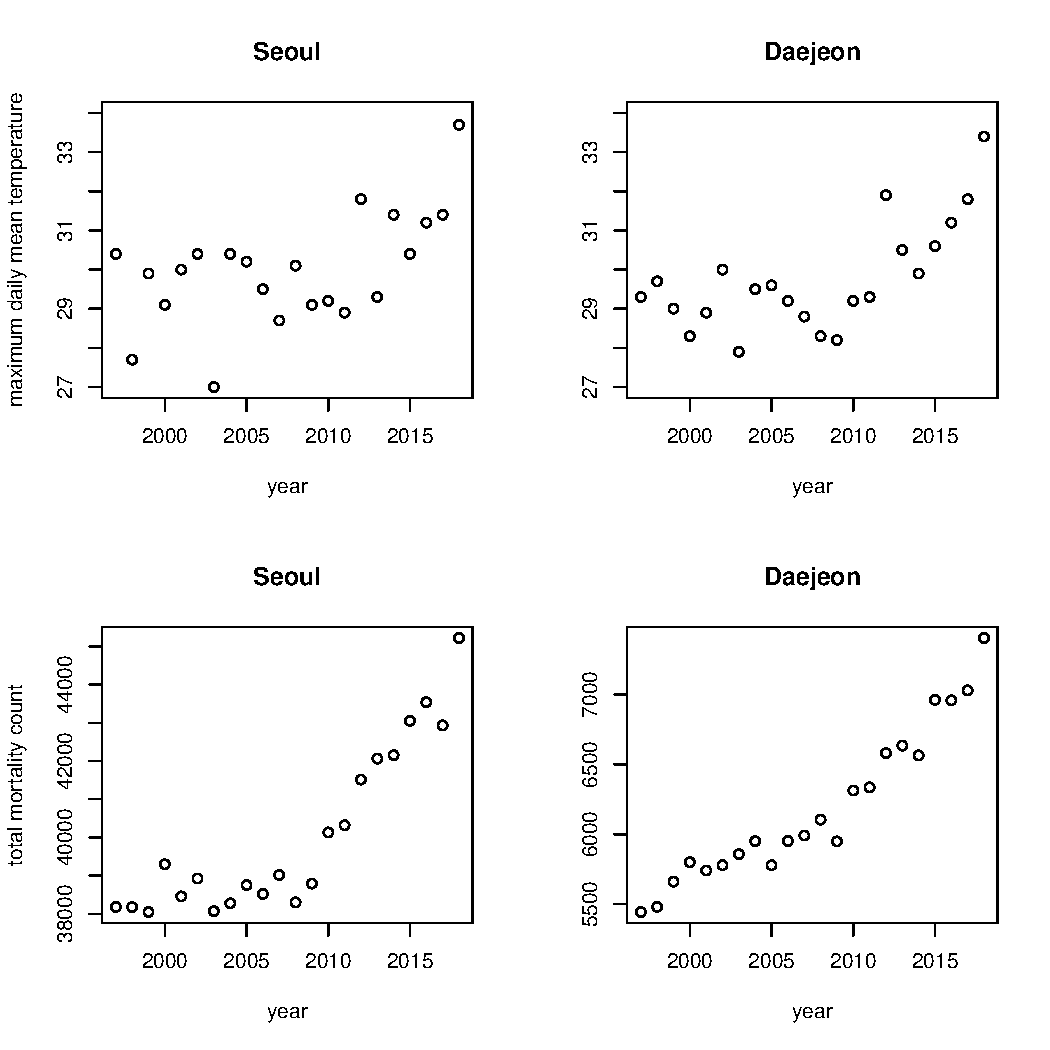
\includegraphics[width = \textwidth]{figures/temporal-trend.pdf}
	\caption{
		Daily times series of 
		mean temperature (in Celcius) and all-cause death in Seoul from 2010 to 2018}
	\label{figure:temporal-trend}
\end{figure}


\section{Method} 
\label{section:method}

For $i = 1, \dots, N(=36)$ and $t = 1, \dots, T(=8054)$, 
the information of $i$-th region at time $t$ can be described by $(Y_{i,t}, W_{i,t}, C_{i,t})$ 
where $Y$ is the all-cause death counts, $W$ is the mean temperature, 
and $C$ is the vector of the year, the month of year, the week of year, and the day of year.
Hereafter, we consider a fixed region and drop the subscript $i$ to simplify the notation.

\subsection{Distributed Lag Nonlinear Model}
\label{section:dlnm}

In the DLNM framework,
the temperature-mortality association is described by the equations
\[
	\begin{split}
		Y_t &\sim quasi-Possion(\lambda_t), \\
		\log(\lambda_t) &= \alpha + cb(W_t, \dots, W_{t-L};\beta) + \eta(C_t; \gamma).
	\end{split}
\]
where $\lambda_t$ is the mean of 
the Poisson distribution with overdispersion (namely, Quasi-Possion\cite{quasipoisson}),
$cb$ is the cross basis function with specified lag $L$,
and $\eta$ is spline basis.
By maximizing quasi-likelihood function, 
we get estimates $\hat{\alpha}, \hat{\beta}$ and $\hat{\gamma}$.
Here, we emphasize that 
including $\eta$ in the model is equivalent to eliminating temporal trend in all-cause deaths
to see the short term variation,
and fitting $cb$ function is estimating temperature effect,
thus the design stage \& the analysis stage are mixed.


\subsection{Rubin Causal Model}
\label{section:rcm}

Now we introduce the notation of potential outcomes.
$Y_t(w)$ refers to the outcome variable at time $t$
that would have been observed under the treatment value $W_t = w$.
$Y_t(w')$ is the outcome variable that would have been obeserved by the counterfactual imagination
that $W_t = w'$ had been observed instead of $W_t = w$.
Observed outcome $Y_t$ is equal to the potential outcome under observed treatment value, $Y_t(W_t)$.
This is called consistency assumption \ref{asm:consistency}.
See the reference\cite{whatif2020} for more detailed explanation about the definition.

We might be interested in the individual risk ratio
\[
	\frac{Y_t(w)}{Y_t(w')}
\]
if we know true values of $Y_t(w)$ and $Y_t(w')$.
However, we never know the true potential outcomes of unmeasured treatment, 
due to its counterfactual nature.
This is called the fundamental problem of causal inference\cite{holland1986}.
Instead, we concentrate on the average risk ratio
\[
	\frac{\mathbb{E}\left[ Y_t(w) \right]}{\mathbb{E}\left[ Y_t(w') \right]}.
\]
There has been many studies to estimate $\mathbb{E}[Y_t(w)]$.
In marginally randomized experiment, 
$\mu(w) = \mathbb{E}[Y(w)]$ can be estimated from observed data\cite{rubin1974}.
In observational studies, 
one can estimate causal estimand $\mu(w)$ by preprocessing the data to approximate randomization 
e.g., inverse probability weighting, standardization, matching\cite{rosenbaum1983}.
Note that we dropped the subscript $t$ to indicate more general situation than time-series setting.
Throughout those techniques, 
the fundamental assumptions that make it possible to estimate the causal estimand are below:

\begin{asm}[Consistency]\label{asm:consistency}\hfill

	Potential outcome for observed treatment is equal to the observed outcome.
	That is, $Y_t(W_t) = Y_t$.
\end{asm}

\begin{asm}[Positivity]\label{asm:positivity}\hfill

	Discrete treatment:
	For all $w$ and $C_t$, $p(w\lvert C_t) = Pr\left ( W_t = w \lvert C_t\right ) \in (0, 1)$.

	Continuous treatment:
	For all $w$ and $C_t$, $p(w\lvert C_t) > 0$ where $p(w\lvert C_t)$ is a conditional density.
\end{asm}


\begin{asm}[Weak Unconfoundedness]\label{asm:unconfoundedness} \hfill

	For all $w$, $Y_{t}(w) \perp W_t \lvert C_t$.
\end{asm}


Positivity assumption says all treatments are possible for each confounder.
Weak unconfoundedness assumption, 
also known as "weak ignorability" or "selection on observables" in different context, says
conditional on current confounders, assignment mechanism is random to potential outcomes.
Under these three assumptions, the causal estimand can be calculated as
\[
	\begin{split}
		\mathbb{E}\left[ Y_t\frac{1_{(W_t = w)}}{p(w\lvert C_t)} \right]
		& = \mathbb{E}\left[ \mathbb{E}\left( Y_t(w) \frac{1_{(W_t = w)}}{p(w\lvert C_t)} \lvert C_t\right)\right]\\
		& = \mathbb{E}\left[ Y_t(w)\frac{\mathbb{E}\left( 1_{(W_t = w)}\lvert C_t \right)}{p(w\lvert C_t)} \right]\\
		& = \mathbb{E}\left[ Y_t(w) \right] = \mu(w),
	\end{split}
\]
where $p$ is a mass or density function for discrete or continuous treatment respectively.
The first equality comes from the interated expectation formula and assumption \ref{asm:consistency},
the second equality comes from assumption \ref{asm:unconfoundedness},
and the third equality is due to the definition of $p(w\lvert C_t)$.
Thanks to the assumption \ref{asm:positivity}, we can divide by $p(w\lvert C_t)$.
This is called "inverse probability weighting" (IPW)
which is used to approximate randomized experiment from conditionally randomized experiment.
Therefore, a natural estimator of the causal estimand is
\[
	\hat{\mu}(w) = \frac{1}{T}\sum_{t = 1}^T Y_t \frac{1_{(W_t = w)}}{p(w\lvert C_t)}.	
	(Consistency???)
\]

Still, we need to estimate $p(w\lvert C_t)$ since it is unknown to us in general.
When the treatment is binary, $p(w\lvert C_t)$ is called propensity score,
and it is used to adjust for confounding bias\cite{rosenbaum1983}.
Propensity score can be extended to 
"generalized propensity score" (GPS) for categorical or continuous treatment\cite{imbens2000}.
For binary treatment, one can estimate propensity score by fitting logit model to data.
For categorical or continuous treatment, GPS can be estimated by fitting ordered probit model or boosting.

PS and GPS have two nice properties\cite{rosenbaum1983, hirano2004}.
The first one is balancing property, which means that conditional on the same PS (or GPS),
treatment and covariates are independent.
The second one is PS-unconfoundedness, 
which means that conditional independence of potential outcome and treatment given PS.
PS-unconfoundedness is implied by balancing property and unconfoundedness.
These properties are the basis of propensity score based matching methods.
But in this paper, 
we used inverse probability weighting so these properties are not necessary to be explained more.

The main reason why we use inverse probability weighting by GPS is to achieve covariate balance.
In randomized experiment, distribution of covariates are similar across each treated group.
However, we are now dealing with observational data which is not randomized.
So, we generate a pseudo-population by imposing appropriate weights to each observation
and look forward to the pseudo-population achieve covariate balance.
One criteria for covariate balance is the absolute correlation (AC)\cite{gpsboosting2015}.
If treatment and covariates are independent, then their correlation must be zero.
So, small value of AC can be an evidence of covariate balance.
Usually, AC with $ <0.1 $ is considered as acceptible.


\section{Application}
\label{section:application}

We set the reference temperature by $20^\circ$C.
\subsection{Distributed Lag Nonlinear Model}

We fitted the DLNM to our data to obtain region specific effect estimates.
Based on the previous study\cite{gasparrini2015},
we used quadratic B-spline, and placed knots at 10th, 75th, 90th quantiles
for temperature dimension,
we considered $21$ lags, used natural B-spline, 
and placed $3$ knots at equally spaced values in the log scale for lag dimension
for lag dimension,
we fitted additional natural B-spline with $8$ degrees of freedom for each year
to eliminate seasonality,
and indicator variables of the day of week was included to control its effect.

With multiple effect estimates from various reigions,
we pooled those estimates by multivariate meta-analysis.
We modeled effect estimates $\hat{\beta}_i$ from $i$-th region as a mixed-effect model
\[
	\hat{\beta}_i \sim N_m(\beta, S_i + V)
\]
where $N_m$ denotes $m$-dimensional multivariate normal distribution,
$S_i$ and $V$ are with-in and between study error covariances, respectively,
and $\beta$ is the true aggregated effect.
We used R package 'mixmeta' to estimate $\beta$ and its confidence interval.
See the upper left panel of figure \ref{figure:main}.

\subsection{Rubin Causal Model}

We rounded daily mean temperature to integer value.
The first stage is design stage to adjust for time confounding.
We adjusted confounding bias by stabilized inverse probability weighting\cite{sipw2010}
that assign weights
\[
	q_t = \min{ \left \{ \frac{\hat{p}(W_t)}{\hat{p}(W_t \lvert C_t)}, 10 \right \} }
\]
to each obsevation.
Here, we don't know true probability densities,
so we should use estimated values.

To estimate $p(W_t \lvert C_t)$, 
we assumed that 
the conditional distribution of treatment given covariates is a normal distribution, i.e.
\[ 
	W_t\lvert C_t \sim N(m(C_t), \sigma(C_t)^2) 
\] 
where $m(C_t)$, and $\sigma(C_t)$ are some functions of $C_t$.
Obviously, there might be more predictors than the date,
but we considered their influence as a Gaussian error term based on the central limit theorem.
Since they are unknown in general, we should estimate them. 
The estimated mean $\hat{m}(C_t)$ was obtained by regressing $W_t$ on $C_t$ with boosting, 
and the estimated standard deviation $\hat{\sigma}(C)$ was calculated
by boosting residuals\cite{hirano2004, gpsboosting2015}.
Hyperparameters such as depth of tree($3$), shrinkage($0.1$), and the number of trees($20$) 
were determined heuristically to minimize the absolute correlation.
As an estimate of $p(W_t)$, we used relative frequency as $\hat{p}(W_t)$.
One may use normal density with sample mean and sample variance too, but
weighting method with relative frequency achieved lower absolute correlation in this application.
See the second row and third row of Table 1.
We trimmed weights bigger than $10$ by $10$,
because some untrimmed weights were too large so
effect estimate was heavily dependent to those observations.

We calculated absolute correlation (AC)\cite{gpsboosting2015} 
to see whether the covariate balance is achieved (here, AC $<0.1$).
Let $c_t$ be a component of $C_t$, then absolute correlation with weight $q_t$ is
the absolute value of Pearson correlation coefficient between $c_t$ and $W_t$,
regarding each observation as $q_t$ observations with the same values.
See the table \ref{table:AC}.

\begin{table}[ht]
	\centering
\begin{tabular}{|| c || c | c | c | c || }
	\hline\hline
	\ & year & month & week of the year & day of the year \\
	\hline
	1 & 0.01405874 & 0.25223312 & 0.25127380 & 0.25115386 \\ %0.43699789 before
	\hline
	2 & 0.03168787 & 0.08356729 & 0.08222320 & 0.08186817 \\ %0.45999471 after
	\hline
	3 & 0.03033376 & 0.12613061 & 0.12417815 & 0.12356290 \\ %0.42005983 normal marginal
	\hline\hline
	
\end{tabular}
\caption{
	Absolute correlation (AC) before/after adjustment by IPW.
	The first row is AC before adjustment;
	the second row is AC after adjustment, 
	with relative frequency of temperature as marginal probability;
	the third row is AC after adjustment, 
	with normal assumption on marginal distribution of temperature.}
\label{table:AC}
\end{table}

The second stage is the analysis stage that relates treatments and outcomes with weights.
We estimated the causal effect by Horvitz-Thompson estimator with trimmed stabilized weights,
\[
	\hat{\mu}(w) = \frac{\sum_{t = 1}^T q_t Y_t 1_{(W_t = w)}}{\sum_{t = 1}^T q_t 1_{(W_t = w)}}.
\]

To be consistent with previous studies and standardize different population size across regions,
we calculated logRR curve by $\log\hat{\mu}(w) - \log \hat{\mu}(20)$ instead of risk difference.
However, there is no known result about the distribution of estimator of risk ratio.
So we measured the uncertainty of logRR curve by Moving Block Bootstrapping (MBB)\cite{mbb1989}
with $2000$ bootstrap samples, $20$ blocks, and each block is length of $400$.
In the bootstrap procedure, we did not fit gps model repeatedely for each bootstrap sample
since we need to re-sample the pseudo-population itself that acheives covariate balance.

To pool the estimates,
we assumed $X_i = (Y_{i,t}, W_{i,t}, C_{i,t})_{t = 1}^T$ for $i = 1, \dots, N$ are independent
and potential outcomes of one region is independent of other regions' potential outcomes and treatments.

We estimated $\hat{\mu}_i(w)$ for each region $i$ previously.
To obtain aggregated estimate, we assumed
\[
	\hat{\mu}_i(w) = \mu(w) + \epsilon_i + \tau,
\]
where $\epsilon_i \sim N(0, s_i)$ is within study error and $\tau \sim N(0, v)$ is between study error.
$s_i$ is estimated by bootstrap,
so estimation of $v$ remains.
We estimated $v$, and aggregated estimates from 36 regions
by taking weighted average of region specific effect estimates
where weight is inversely proportional to the variance $s_i + v$ of estimator,
\[
	\hat{\mu}(w) = \sum_{i = 1}^N \frac{\hat{\mu}_i(w)}{s_i + \hat{v}}
	/\sum_{i = 1}^N \frac{1}{s_i + \hat{v}}.
\]
Precision of pooled estimator is sum of precisions of region specific estimator,
\[
	\frac{1}{\hat{\sigma}^2} = \sum_{i = 1}^N \frac{1}{s_i + \hat{v}}.
\]
Confidence interval is obtained by 
\[
	\hat{\mu}(w) \pm 1.96 \hat{\sigma}.
\]
See the upper right panel of figure \ref{figure:main}.


\subsection{Result}

\begin{figure}
	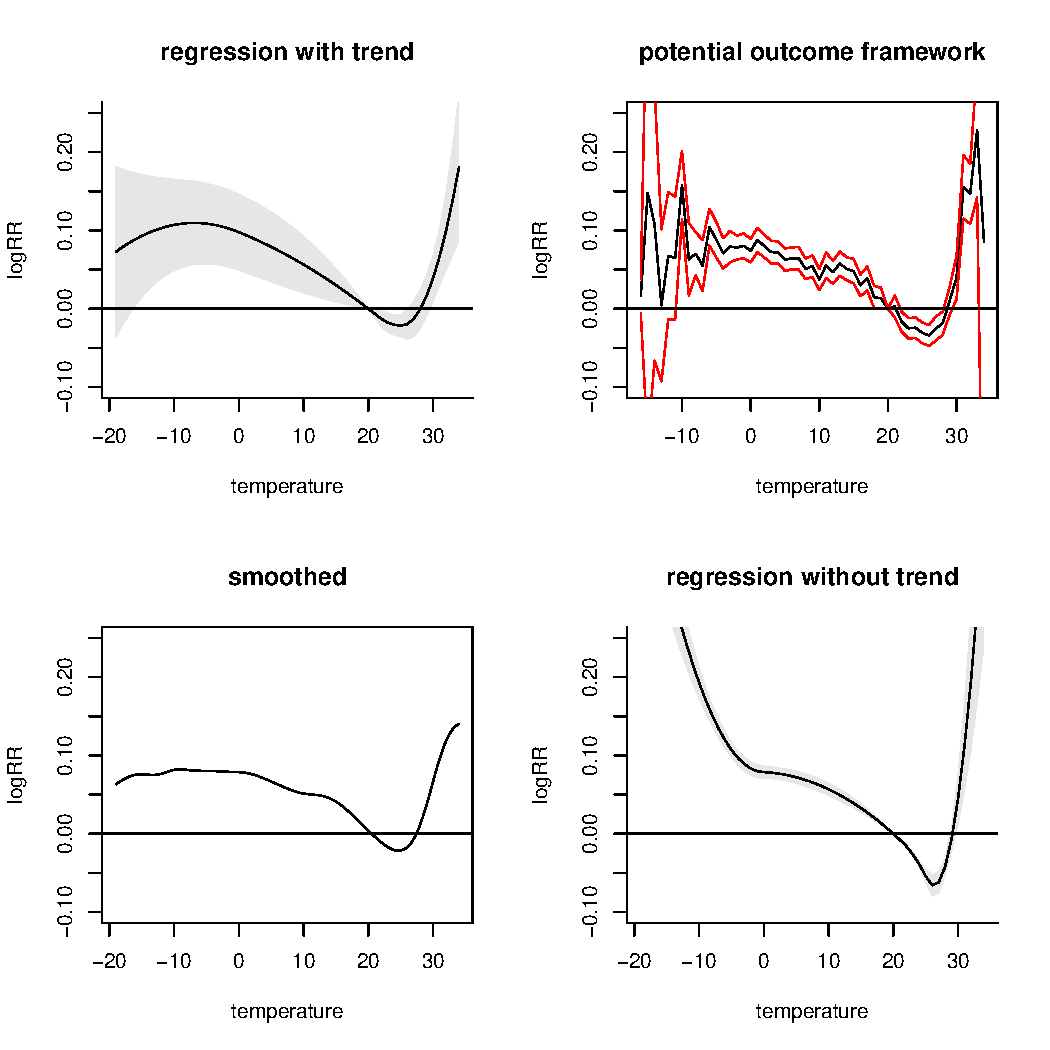
\includegraphics[width = \textwidth]{figures/main1.pdf}
	\caption{Estimated overall effect. 
	For extreme hot or cold temperature, estimated effects have quite large uncertainties.}
	\label{figure:main}
\end{figure}

In figure \ref{figure:main},
the upper left panel is a logRR curve obtained under the DLNM framework;
the upper right panel is obtained by applying RCM;
the lower left panel is smoothed version of upper right pannel (kernel: Gaussian, bandwidth: $6$);
the lower right pannel is a logRR curve without adjusting temporal trend under the DLNM framework.

The estimated logRR curve of the lower right panel has exaggerated values at extreme temperatures,
compared to the upper left panel.
Since the model of the lower right panel does not consider temporal trend,
the difference between two panels comes from autocorrelation of outcome variable.

The logRR curve of the upper right panel is spiky,
because we estimated it by model free method, so it heavily depends on the observations.
For the most cold temperature, 
we can see that the confidence interval is narrow compared to the most hot temperature.
This is because there is only one such observation,
so uncertainty captured by bootstrap is due to the variation of effect estimate at the reference temperature.

In the lower left pannel, we applied kernel smoothing to our estimate to remove spikes.
The smoothed curve and the curve of the upper left panel have similar values 
compared to the curve of the lower right panel.
From this point of view, 
we may say RCM can adjust temporal confounding bias in some extent.
Moreover, we don't know what is the true logRR curve,
but we may insist that the logRR curve obtained from RCM is more general
in the sense that it becomes similar to the curve of DLNM after kernel smoothing.


\section{Discussion}
\label{section:discussion}

In this article,
the DLNM framework and Rubin causal model were compared
to discover a causal link between the ambient temperature and all-cause mortality.
In the extent of my knowledge, there has been no study analyzing the short term relationship 
between the ambient temperature and the all-cause mortality using RCM.
Two pooled results obtained via two different methods
showed similar effects of the ambient temperature, after smoothing.
This similarity, or consistency
added an evidence of causal relationship found by previous studies.

(단점 나열, 어떻게 극복했는지)

In RCM, we could not do several analyses that the DLNM framework can do:
identification of the lagged effect, 
distribution based confidence interval, and multivariate meta-analysis.
The exposure-response surface that the DLNM framework produces 
makes us possible to identify lagged effect of the ambient temperature.
In contrast, RCM does not have ability to measure the lagged effect of the ambient temperature,
since it does not use any information about lagged temperature.
Indeed, there is a method to measure the lagged effect of binary treatment in RCM\cite{bojinov2019},
but the curse of dimension inhibits direct application of that method to our case.
\begin{comment}
	%Controversial: 
Someone may say to us that the calculated logRR curve does not represent overall effect 
but represents instant effect since we did not account for lagged effect.
However, under the assumption that 
treatment history would have been almost the same during short period, due to their high autocorrelation,
our effect estimate represents overall effect.
\end{comment}
The DLNM framework provides the confidence interval based on asymptotic normality 
followed by maximizing quasi-likelihood function.
Unfortunately, there is no exact or asymptotic distribution of our estimator in our case,
due to the difficulty derived from the definition of RR, 
which is the ratio between two effects, not the difference.
So we quantified the uncertainty of estimated logRR curve by moving block bootstrap.
Moreover, the standard error of pooled logRR curve seems not similar to the one from the DLNM framework.
This is because,
the precision of overall effect was obtained by summing up all precisions from each region,
but some regions did not have observations of extremal temperature.
This leads us to relatively low precision of overall effect estimates in extreme temperature.
The heterogeneity of temperature effect has been explained by multivariate meta-analysis
that has spline coefficients obtained from the DLNM framework as the response variable, 
and regional level variables such as latitude or climate zone as meta-predictors.
Loosely speaking, multivariate meta-analysis with coefficients that summarize the estimated RR curve
is analyzing the heterogeneity of curve itself across regions.
However, in our suggestion, we just pooled the effect estimates from each region pointwisely.
In fact, multivariate meta-analysis is possible by considering bootstrap covariance,
but it is computationally too expensive.

In addition to the weekness compared to the regression method stated above,
our method has disadvantages of itself to be addressed:
incorrect treatment assignment mechanism, and violation of assumptions.
We predicted daily mean temperature with only date,
in spite of the existence of other factors such as 
cloud, rain, air mass, typhoon, CO2 emission, global warming, etc,
because the primary factor that determines daily mean temperature is the meridinal altitude.
So the assignment mechanism we assumed was theoretically incorrect,
but can be improved by including other factors that are able to predict the temperature into GPS model.
\begin{comment}
	% variance-bias tradeoff, might be inappropriate
We estimated logRR curve without any modeling assumption after confounding adjustment.
Also, the estimator does not borrow information near given treatment value.
This makes the estimate soley rely on observed values.
However, we have few observations for extreme temperature.
So few observations play an important role in effect estimating procedure,
and it means our approach may have high variance and low bias.
It is the same for previous studies that there are only few extreme temperature observations,
but they assumed parametric model to the outcome generating process
so effect estimates at extreme temperature is a result of borrowing information near the temperature point,
and it makes extreme cases play somewhat shrinked role compared to our approach,
which means lower variance and higher bias.
\end{comment}
There is a possibility of violation on 
two key assumptions \ref{asm:positivity},\ref{asm:unconfoundedness} in RCM.
The first one is positivity assumption
that any treatment has positive probability of being assigned for each confounder.
In our case, the confounder is time and 
there is always nonzero probability of extreme temperature because of catastrophic events.
However those events rarely happen in reality, 
so stochastic positivity violation\cite{zivich2022} due to small sample size can happen.
To fix the issue, we made normal assumption on gps,
and trimmed very small probability to $0.1$ to ensure stability.
The second one is (weak) unconfoundedness
that may be violated when there is an unmeasured confounder.
In our case, we cannot measure everything related to temperature-mortality relationship
so it is plausible to think the assumption \ref{asm:unconfoundedness} is violated.
To overcome this issue, we should carefully think about confounding structure
and collect more data of potential confounders.


\bibliography{reference}{}
\bibliographystyle{plain}


\end{document}
